\documentclass[10pt,xcolor={svgnames}]{beamer}

%%%%% Colors
\usetheme{Dresden}%\usetheme{Madrid}
\colorlet{beamer@blendedblue}{green!55!black}
%%%%%

%%%%% Other 
\addtobeamertemplate{navigation symbols}{}{%
    \usebeamerfont{footline}%
    \usebeamercolor[fg]{footline}%
    \hspace{1em}%
    \insertframenumber/\inserttotalframenumber
}
\usepackage{hyperref, url}

\definecolor{pine_green}{HTML}{007935}
\hypersetup{colorlinks,breaklinks,linkcolor=white,urlcolor=orange,citecolor=black}
\renewcommand\thefootnote{\textcolor{pine_green}{\arabic{footnote}}}
\setbeamercolor{alerted text}{fg=pine_green}

\usepackage{cancel}
\usepackage{ulem}
\usepackage{multirow}
\usepackage{mathtools}
\renewcommand{\epsilon}{\varepsilon}
\setbeamertemplate{itemize subitem}{\textbullet}
\setbeamertemplate{itemize subsubitem}{$\circ$}

%https://tex.stackexchange.com/questions/289542/auto-resizing-parenthesis-in-math-formulas
% \usepackage{amsmath} for testing
\newcommand*\autoop{\left(}
\newcommand*\autocp{\right)}
\newcommand*\autoob{\left[}
\newcommand*\autocb{\right]}
\AtBeginDocument {%
   \mathcode`( 32768
   \mathcode`) 32768
   \mathcode`[ 32768
   \mathcode`] 32768
   \begingroup
       \lccode`\~`(
       \lowercase{%
   \endgroup
       \let~\autoop
   }\begingroup
       \lccode`\~`)
       \lowercase{%
   \endgroup
       \let~\autocp
   }\begingroup
       \lccode`\~`[
       \lowercase{%
   \endgroup
       \let~\autoob
   }\begingroup
       \lccode`\~`]
       \lowercase{%
   \endgroup
       \let~\autocb
   }}

\delimiterfactor 1001

\makeatletter
% for amsmath "compatibility" (not sophisticated)
% \usepackage{amsmath}
\AtBeginDocument {%
          \def\resetMathstrut@{%
           \setbox\z@\hbox{\the\textfont\symoperators\char40}%
           \ht\Mathstrutbox@\ht\z@ \dp\Mathstrutbox@\dp\z@}%
}%
\makeatother
%%%%%

%%%%% Greying out/invidible Slides
%\setbeamercovered{invisible}
%\setbeamercovered{%
%  again covered={\opaqueness<1->{15}}}
  
%%%%%







%%%%% Footnotes and captions
%\usepackage[utf8]{inputenc}
\usepackage{caption}
\usepackage{comment}
\setbeamerfont{footnote}{size=\tiny}
\setbeamerfont{caption}{size=\small}
%\setbeamerfont{normal text}{size=\small}
\setbeamerfont{itemize/enumerate body}{size=\small}
\setbeamerfont{itemize/enumerate subbody}{size=\footnotesize}
%%%%%



%Information to be included in the title page:
\title[Connor Wiegand]{Intro to Economic Analysis: Microeconomics}
\subtitle{EC 201 - Day 5 Slides}
\author[EC 201]{Connor Wiegand}
\institute[]{Department of Economics - University of Oregon}
\date{11 October 2021}


\begin{document}

\frame{\titlepage}

\begin{frame}{Logistics}
    \begin{itemize}
        \item Official homework 2 due this Saturday at 11:59pm, covering last week's material
        \item News assignments posted, first one due this Wednesday (October 13)
        \begin{itemize}
            \item This includes doing 1 news analysis of your choice on Cengage, \underline{and}
            \item Submitting a 1-1.5 page write up on Canvas
        \end{itemize}
        \item The outline must contain a brief summary of the article you read, as well as responses to the discussion questions that were at the end of your Cengage News Analysis    
        \end{itemize}
\end{frame}

\section*{Single Shifts}

\begin{frame}{Recap of last week}
    \begin{itemize}[<+->]
        \item Recall our shifters for supply and demand
        \item For supply...
        \begin{itemize}
            \item changes in price of inputs
            \item changes in technology
            \item changes in \# of sellers in the market
            \item changes in expectations
            \item And natural disasters
        \end{itemize}
        \item For demand...
        \begin{itemize}
            \item changes in income
            \item changes in tastes and preferences
            \item changes in \# of market participants
            \item changes in expectations
            \item changes in the price of related goods
        \end{itemize}
    \end{itemize}
\end{frame}

\begin{frame}{Single Shifts}
    \begin{itemize}[<+->]
        \item So what effects do these shifts have on the market?
        \item Specifically, suppose the market is in equilibrium, what effect does a change in demand bring? What about a change in supply? Will the effect always be the same?
    \end{itemize}
\end{frame}

\begin{frame}{Framework}
    \begin{itemize}[<+->]
        \item Suppose the market for pizza is in equilibrium, as shown in the diagram below:
    \end{itemize}
\end{frame}

\begin{frame}{Example 1}
    \begin{itemize}[<+->]
        \item Suppose that TotallyReliable Health Magazine announces that eating pizza every day reduces your chances of heart disease by 20\%. What happens in the supply and demand graph? What happens to the equilibrium price and quantity?
        \item Since  pizza is believed to be healthier (taste and preferences) goes up, demand will shift right
    \end{itemize}
\end{frame}

\begin{frame}{Example 1 (cont.)}
        \begin{table}[]
            \centering
            \begin{tabular}{c}
            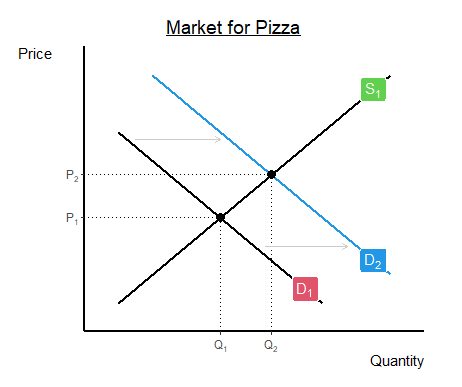
\includegraphics[width=6.5cm]{DR.png}
            \end{tabular}
            \caption*{As we can see in the diagram, this will cause the price of pizza to rise in equilibrium, and will also increase the equilibrium amount of pizza being traded}
        \end{table}
\end{frame}

\begin{frame}{Example 2}
    \begin{itemize}[<+->]
        \item Suppose instead that the price of ranch skyrockets, making it accessible to only the top 0.1\% of Americans. Now what happens in equilibrium?
        \item Since ranch is a complement to pizza\footnote{like it or not}, demand for pizza will fall
    \end{itemize}
\end{frame}

\begin{frame}{Example 2 (cont.)}
        \begin{table}[]
            \centering
            \begin{tabular}{c}
            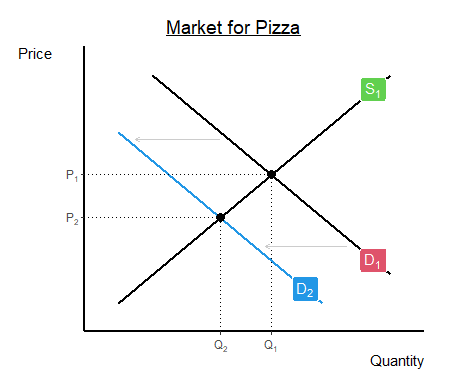
\includegraphics[width=6.5cm]{DL.png}
            \end{tabular}
            \caption*{This causes the price of pizza to fall, as well as the equilibrium quantity}
        \end{table}
\end{frame}

\begin{frame}{Example 3}
    \begin{itemize}[<+->]
        \item Now suppose that instead of either of these changes, the price of cheese increases. Now what happens in equilibrium?
        \begin{center}
            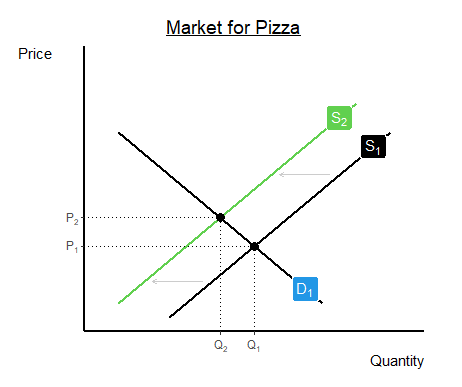
\includegraphics[width=6cm]{SL.png}
        \end{center}
        \item The supply of pizza will shift left, and we can see that the price of pizza rises, while the quantity falls
    \end{itemize}
\end{frame}

\begin{frame}{Example 4}
    \begin{itemize}[<+->]
        \item Suppose instead that people start fleeing New York, and many of them want to open up NY Pizza joints. Now what happens in equilibrium?\vspace{-0.5mm}
                \begin{center}
            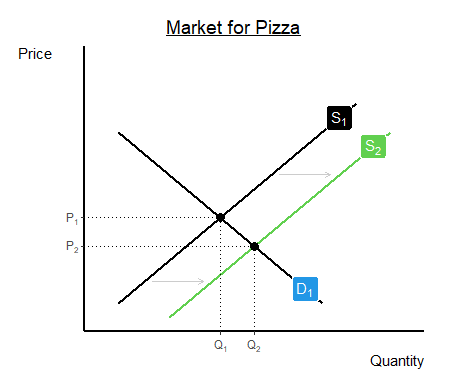
\includegraphics[width=6cm]{SR.png}
        \end{center}\vspace{-0.5cm}
        \item Supply shifts right due to increased producers, and we can see that the price of pizza falls and equilibrium quantity rises 
    \end{itemize}
\end{frame}

\begin{frame}{Effects of Different Kinds of Shocks}
    \begin{itemize}[<+->]
        \item Intuition behind supply/demand increases:
        \begin{itemize}
            \item $[D]$ When a product or market takes off in terms of demand, the suppliers will increase the price to match the rise in demand, which often includes ramping up production, which can be costly
            \item $[S]$ When a firm gets better technology, they can produce product for cheaper and/or increase more of it; this allows them to lower the price so they can sell more from the increased production
        \end{itemize}
        \item Which is your favorite?
        \item Positive supply shocks\footnote{Shock is a common term used by economist to mean change in the model} are generally favorable (to consumers), since they lower the price and the overall quantity, in equilibrium
        \item However, one can imagine that when done at a large scale, stimulating/pulling back one of these curves can have economy-wide effects (macroeconomic effects)
        \item This can also have different welfare effects on both consumers and producers, which is the direction we will head in next week
    \end{itemize}
\end{frame}

\begin{frame}{Summary}
    \begin{itemize}[<+->]
        \item To summarize:
        \begin{itemize}
            \item Demand
            \begin{itemize}
                \item Increase: price up, quantity up
                \item Decrease: price down, quantity down
            \end{itemize}
            \item Supply
            \begin{itemize}
                \item Increase: price down, quantity up
                \item Decrease: price up, quantity down
            \end{itemize}
        \end{itemize}
    \end{itemize}
\end{frame}

\section*{Double Shifts}

\begin{frame}{Double Shifts in Supply and Demand}
    \begin{itemize}[<+->]
        \item Now that we have gone through shifting one curve at a time, what happens when we shift two curves at once?
        \item Consider the following example in the market for seltzers:
        \begin{itemize}
            \item Suppose that beer regulations tighten, and causing the price of beer to rise
            \item At the same time, the U.S. puts restrictions on aluminium trade, causing its price to rise
        \end{itemize}
        \item What will happen to market equilibrium?
    \end{itemize}
\end{frame}


\begin{frame}{Example 4}
    \begin{itemize}[<+->]
        \item First off, what will happen to supply \& demand?
        \begin{itemize}
            \item Demand will shift right
            \item Supply will shift left
        \end{itemize}
        \item Let's visualize this
    \end{itemize}
\end{frame}

\begin{frame}{Example 4 (cont.)}
\begin{center}
    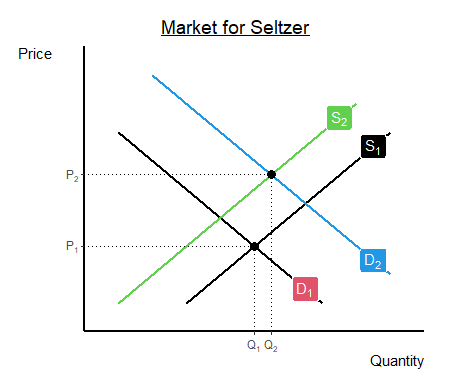
\includegraphics[width=6cm]{SL_DR1.png}
\end{center}
    \begin{itemize}[<+->]
        \item In this graph, both the equilibrium quantity and equilibrium price rose
        \item But recall that these are abstract shifts, i.e. without numbers. What happens if we were to draw it differently?
    \end{itemize}
\end{frame}

\begin{frame}{Example 4 (cont.)}
\begin{center}
    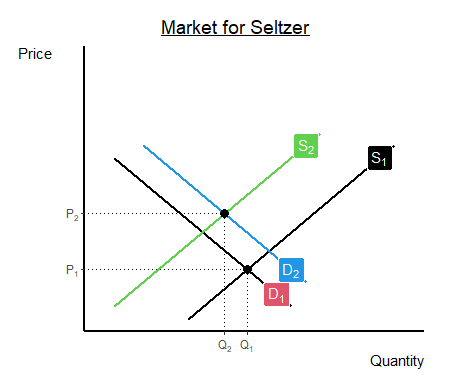
\includegraphics[width=7cm]{SL_DR2.png}
\end{center}
    \begin{itemize}[<+->]
        \item \vspace{-2mm} Now, equilibrium price rises but equilibrium quantity falls
    \end{itemize}
\end{frame}

\begin{frame}{Example 4 (cont.)}
\begin{center}
    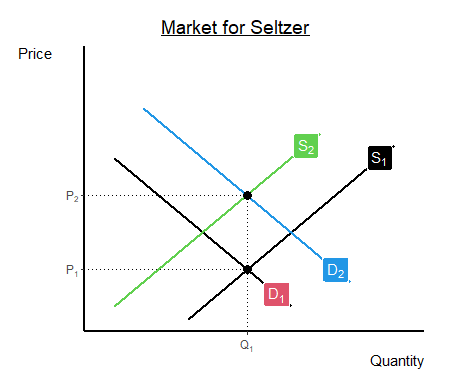
\includegraphics[width=7cm]{SL_DR3.png}
    \vspace{-6mm}
\end{center}
    \begin{itemize}[<+->]
        \item Now, equilibrium price rises but equilibrium quantity doesn't even move
        \item What's the deal?
    \end{itemize}
\end{frame}

\begin{frame}{Shifting Two Curves at Once}
    \begin{itemize}[<+->]
        \item When shifting two curves at once (without numbers)\footnote{if we have numbers and equations, we can of course calculate the actual equilibria}, there will always be one equilibrium object that we can determine, and one which we cannot
        \item Example: in the above diagram, which equilibrium object always moved in the same direction?
        \begin{itemize}
            \item A: Price, which always rose
        \end{itemize}
        \item You can draw the above diagram such that quantity rises, falls, or stays the same, but price will always rise, as long as you preserve shapes (you are welcome to try to draw it such that this isn't the case)
    \end{itemize}
\end{frame}

\begin{frame}{How to Determine Equilibria Direction}
    \begin{itemize}[<+->]
        \item So how do we figure out which object is determined (and what direction it moves in), and which is ambiguous?
        \item One idea is to just draw a bunch of curve shifts of various sizes, and analyze which of price/quantity always moves in the same direction, and which can move in either direction
        \item This may be a good idea if you forget which is which, but there is a more analytical way to determine which is which
    \end{itemize}
\end{frame}

\begin{frame}{How to Determine Equilibria Direction (cont.)}
    \begin{itemize}[<+->]
        \item Recall the previous example, in which demand shifted right and supply shifted left
        \item Note:
        \begin{itemize}
            \item D$\uparrow\ \implies\ P\uparrow\ \& \ Q\uparrow$
            \item S$\hspace{0.5mm}\downarrow\ \implies\ P\uparrow\ \& \ Q\downarrow$
        \end{itemize}
        \item Thus, both shifts that occur increase the price, which is why price increases
        \item However, each shift moves quantity in a different direction, meaning a larger shift from either curve can influence the final direction of the change in quantity
        \item Writing these down for any multi-shift example can help you determine which price/quantity moves
    \end{itemize}
\end{frame}

\begin{frame}{Example 5}
    \begin{itemize}[<+->]
        \item Now suppose that the youths convince all of their friends that drinking seltzers is the hip, cool thing to do. To account for this, every beer brewer and their sibling start making a seltzer
        \item What impact does this have on equilibrium?
    \end{itemize}
\end{frame}

\begin{frame}{Example 5 (cont.)}
    \begin{itemize}[<+->]
        \item To start, we know that demand moves \_\_\_\_, and supply moves \_\_\_\_
        \begin{itemize}
            \item Right, in response to the taste/preference shock
            \item Right, in response to the increased number of sellers
        \end{itemize}
        \item So, what direction do we predict market equilibrium objects moving?
        \begin{itemize}
            \item D$\uparrow\ \implies\ P\uparrow\ \& \ Q\uparrow$
            \item S$\hspace{0.5mm}\uparrow\ \implies\ P\downarrow\ \& \ Q\uparrow$
        \end{itemize}
        \item We might expect that eq. quantity moves up and eq. price is ambiguous
        \item Let's check by graphing
    \end{itemize}
\end{frame}

\begin{frame}{Example 5 (cont.)}
\begin{center}
    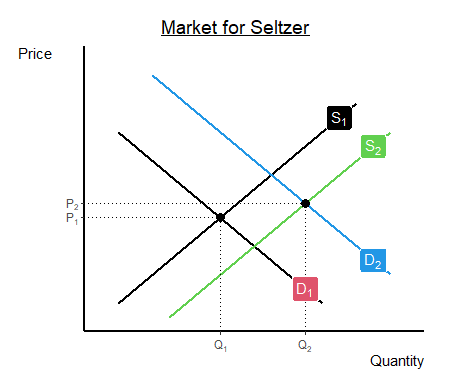
\includegraphics[width=6cm]{SR_DR1.png}
\end{center}
    \begin{itemize}[<+->]
        \item In this graph, both equilibrium quantity and equilibrium price rose
    \end{itemize}
\end{frame}

\begin{frame}{Example 5 (cont.)}
\begin{center}
    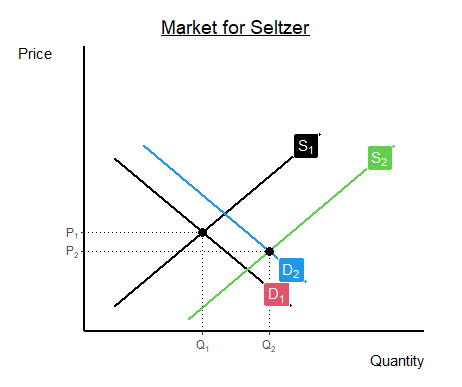
\includegraphics[width=7cm]{SR_DR2.png}
\end{center}
    \begin{itemize}[<+->]
        \item \vspace{-4mm} Now, equilibrium quantity rises but equilibrium price falls
    \end{itemize}
\end{frame}

\begin{frame}{Example 5 (cont.)}
\begin{center}
    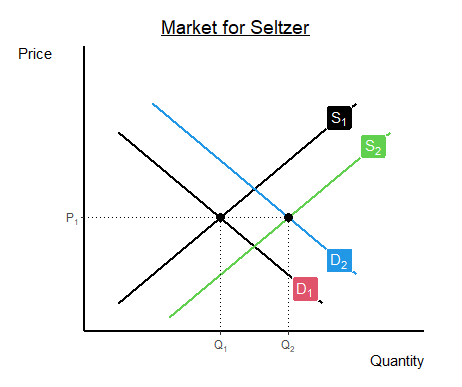
\includegraphics[width=7cm]{SR_DR3.png}
    \vspace{-6mm}
\end{center}
    \begin{itemize}[<+->]
        \item Now, equilibrium quantity rises but equilibrium price doesn't even move
    \end{itemize}
\end{frame}


\begin{frame}{Exercises}
    \begin{itemize}[<+->]
        \item Takeaway: shifting two curves at once will lead to one of price/quantity being known, and the other being unknown
        \begin{itemize}
            \item Again, \underline{assuming you don't have numbers} 
        \end{itemize}
        \item A good exercise and study activity would be checking the other two cases (demand and supply both shifting left, and supply shifting right + demand shifting left) to see the equilibrium effect
        \item Something to think about: what happens if we have more than two shifts?
    \end{itemize}
\end{frame}


\section*{Elasticity}

\begin{frame}{Elasticity}
    \begin{center}
        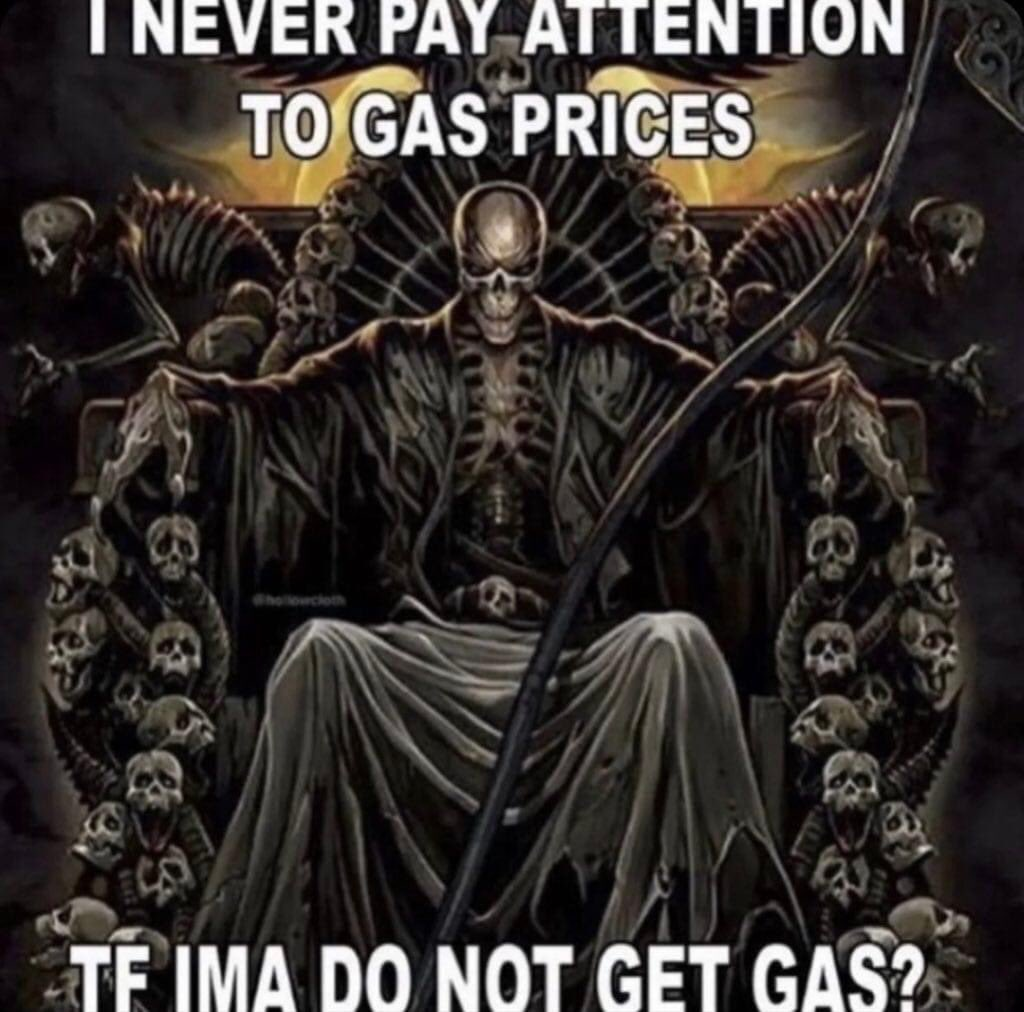
\includegraphics[width=7.35cm]{gas_meme.jpg}
    \end{center}
\end{frame}

\begin{frame}{Rising Prices: Are They All Equal?}
    \begin{itemize}[<+->]
        \item What happens when gas prices rise?
        \item We see a movement along the demand curve, up/left
        \item The result: people demand less gas, according to the law of demand
        \item Separate question: what happens when the price of Captain Crunch rises?
        \item We see a similar movement along the captain crunch demand curve, but do we think it's the same?
        \item Do we think a jump in the price of cereal causes the same loss in quantity demanded as a jump in the price of gas?
    \end{itemize}
\end{frame}

\begin{frame}{Elasticity}
    \begin{itemize}[<+->]
        \item This though experiment gives rise to our next concept: \textit{elasticity}
        \item Informally, elasticity is a measure of how much buyers and sellers respond to changes in market conditions
        \item We will start with types of elasticity of demand, starting with the \textit{price elasticity of demand}
        \item The \underline{\textbf{price elasticity of demand}} measures how much the quantity demanded responds to a change in price
        \begin{itemize}
            \item A good is said to be \textit{inelastic} if consumers are insensitive to changes in price
            \item A good is said to be \textit{elastic} if consumers are sensitive to changes in price
        \end{itemize}
        \item Which do you think gas is?
    \end{itemize}
\end{frame}

\begin{frame}{Price Elasticity of Demand}
    \begin{itemize}[<+->]
        \item Formally, the price elasticity of demand, denoted $e_{d}$, $E_{d}$, or, as I will use, $\epsilon_{D}$, is computed as
        $$\epsilon_{D}=\left|\frac{\%\Delta Q_{D}}{\%\Delta P}\right|$$
        where $\Delta$ is read ``change in"
        \item For example, if I told you that when gas prices rise by 10\%, then quantity demanded for gas falls by 2.5\%, then the PED would be 
        $$\epsilon_{D}=\left|\frac{-2.5}{10}\right|=0.25$$
        \item Before preceding, we have to make some important notes
    \end{itemize}
\end{frame}

\begin{frame}{The Sign of Price Elasticity of Demand}
    \begin{itemize}[<+->]
        \item Recall the law of demand: what happens when the price of a good increases?
        \begin{itemize}
            \item It's quantity demanded decreases
        \end{itemize}
        \item Therefore, what sign will $\frac{\%\Delta Q_{D}}{\%\Delta P}$ have?
        \begin{itemize}
            \item Negative, because an increase in price leads to an increase in $Q_{D}$ and vice versa
        \end{itemize}
        \item However, some\footnote{but not all} economists choose to convert and report $\epsilon_{D}$ as a positive term
        \item The book refers to this as ``common" and simply says they ``drop the negative" -- I want you to know and demonstrate that you know that this is a negative value and we are taking the absolute value (which is the same as dropping a negative)
    \end{itemize}
\end{frame}

\begin{frame}{Calculating Percentage Change}
    \begin{itemize}[<+->]
        \item The second order of business involves the \sout{horrid} atypical way in which we as economists calculate percent change
        \item In the sciences, if $x_{1}$ changes to $x_{2}$, then the percent change in $x$ is given by 
        $$\frac{x_{2}-x_{1}}{x_{1}}\cdot 100\iff\frac{\text{final}-\text{initial}}{\text{initial}}\cdot 100$$
        \item However, using this method, consider a change from $x_{1}=10$ to $x_{2}=80$. What is the percent change in $x$?
        \begin{itemize}
            \item $\%\Delta x=\frac{80-10}{10}\cdot 100=700\%$
        \end{itemize}
        \item But what about the change from 80 to 10?
        \begin{itemize}
            \item $\%\Delta x=\frac{10-80}{80}\cdot 100=-87.5\%$
        \end{itemize}
        \item This lack of symmetry bothered economists so much that they decided to do something completely different\footnote{This is a bit reductive. There are multiple notions of elasticity, one using calculus, and they used an approximation technique to define a new notion of elasticity, the one you are seeing here}
    \end{itemize}
\end{frame}

\begin{frame}{The Midpoint Method}
    \begin{itemize}[<+->]
        \item So, while that way of calculating percentage change might be fine for your science class, here is the formula we will use for calculating percentage change in $x$, again using $x_{1}$ (initial) and $x_{2}$ (final):
        \begin{align*}
            \%\Delta x &= (x_{2}-x_{1})\big/[(x_{2}+x_{1})/2]\cdot 100\\
            &= \frac{x_{2}-x_{1}}{(\frac{x_{2}+x_{1}}{2})}\cdot 100\\
            &= \frac{\text{final}- \text{initial}}{\text{midpoint}}\cdot 100
        \end{align*}
        \item This is called the midpoint method, because we divide the change in $x$ by the midpoint between initial and final
    \end{itemize}
\end{frame}

\begin{frame}{Back to Elasticity}
    \begin{itemize}[<+->]
        \item So, the full formula for elasticity is given by 
        \begin{align*}
            \epsilon_{D}=\left|\frac{\%\Delta Q_{D}}{\%\Delta P}\right|=\left|\frac{(Q_{2}-Q_{1})/[(Q_{1}+Q_{2})/2]}{(P_{2}-P_{1})/[(P_{1}+P_{2})/2]}\right|
        \end{align*}
        \begin{itemize}
            \item 100 cancels from the top and bottom
            \item I drop the letter ``D" from $Q_{D}$ in this case to avoid clutter; \textit{you should only do this when it is clear}
        \end{itemize}
        \item Example: Suppose that when the price of burritos rises from \$8 to \$12, the quantity demanded falls from 1500 to 700. What is the PED for burritos?
    \end{itemize}
\end{frame}

\begin{frame}{Elasticity Example}
    \begin{itemize}[<+->]
        \item When the price of burritos rises from \$9 to \$12, the quantity demanded falls from 1500 to 700
        \begin{align*}
            \epsilon_{D}&=\left|\frac{(700-1500)/[(1500+700)/2]}{(12-8)/[(12+8)/2]}\right|\\
            &=\left|\frac{-800/1100}{4/10}\right|\\
            &=\frac{20}{11}\\
            &=1.\overline{81}
        \end{align*}
        \item What does this say?
    \end{itemize}
\end{frame}

\begin{frame}{PED Interpretation}
    \begin{itemize}[<+->]
        \item Suppose $\epsilon_{D}=1.81$
        \item This says: ``if the price of burritos were to increase by 1\%, then the quantity demanded for burritos would fall by 1.81\%"
        \begin{itemize}
            \item Equivalently, because we are using the midpoint method: ``if the price of burritos were to fall by 1\%, then the quantity demanded for burritos would rise by 1.81\%"
        \end{itemize}
        \item In general, if good $x$ has PED $\epsilon_{D}$, then we would  say ``if the price of $x$ were to increase by 1\%, then the quantity demanded for $x$ would fall by $\epsilon_{D}$\%"
        \item Why? If\footnote{\vspace{1.25mm}Here I am ignoring absolute values, and allowing $\epsilon_{D}$ to be negative, for simplicity} $$\epsilon_{D}=\frac{\%\Delta Q_{D}}{\%\Delta P}$$
        then plugging in $1\%$ for $\%\Delta P$ yields $\epsilon_{D}\%$ for $\%\Delta Q_{D}$:
        $$\epsilon_{D}=\frac{\%\Delta Q_{D}}{\%\Delta P}\implies \epsilon_{D}\%=\%\Delta Q_{D}$$
    \end{itemize}
\end{frame}

\begin{frame}{Types of Elasticity, by Numbers}
    \begin{itemize}[<+->]
        \item Thus, if $\epsilon_{D}<1$ for some good $x$, then we say $x$ is \textit{inelastic}
        \begin{itemize}
            \item Again, this means consumers are insensitive to prices: when prices rise dramatically consumers do not demand much less of the product
        \end{itemize}
        \item If $\epsilon_{D}>1$, we say that $x$ is \textit{elastic}
        \begin{itemize}
            \item Again, this means consumers are sensitive to prices: if prices rise a little bit, then consumers will demand much less of the product
        \end{itemize}
        \item If $\epsilon_{D}=1$, we say that $x$ is \textit{unit elastic}
        \item If $\epsilon_{D}=0$, the $x$ is said to be \textit{perfectly inelastic}
        \begin{itemize}
            \item Consumers are infinitely insensitive to prices, meaning that prices can rise indefinitely and $Q_{D}$ will not be affected
            \item Examples: necessary goods, such as insulin, life-saving medicine, rent (maybe not perfect), etc. 
        \end{itemize}
        \item If $\epsilon_{D}=\infty$, the $x$ is said to be \textit{perfectly elastic}
        \begin{itemize}
            \item Consumers are infinitely sensitive to prices, meaning that the smallest price increase can deplete the whole market of buyers
            \item Examples: goods with many substitutes, or goods which are easily accessible and/or easy to steal; e.g. phone games, souvenirs, any public goods/services with poor monitoring
        \end{itemize}
    \end{itemize}
\end{frame}

\begin{frame}{Determinants of Elasticity}
    \begin{enumerate}[<+->]
        \item Availability of close substitutes
        \begin{itemize}
            \item As aforementioned, if there are a lot of substitutes for a good, then it is likely to have a much higher elasticity of demand: people are more sensitive to the price
            \item Ex: specific meats, such as pork sausage, can be easily substituted for other mets
            \item Ex: Eggs do not have many close substitutes
        \end{itemize}
        \item Necessities vs. Luxuries
        \begin{itemize}
            \item Neccesities, such as insulin, tend to be more price-inelastic, compared to luxuries, such as craft spirits
            \item Other items, which are not ``necessities", can be highly inelastic if they are common-place based on cultural norms, such as phones, computers, wifi, etc. 
        \end{itemize}

    \end{enumerate}
\end{frame}

\begin{frame}{Determinants of Elasticity (cont.)}
    \begin{enumerate}[<+->]
    \setcounter{enumi}{2}
        \item Specificity of the Market
        \begin{itemize}
            \item The specific tiers in the market can influence how sensitive people are to prices. \textit{Generally}, broader markets tend to be more price-inelastic than narrow ones
            \begin{itemize}
                \item E.g. food is necessary, hence price-inelastic, while Ribeye, a specific cut of steak, may be a luxury with close substitutes
                \item Alcohol may be price-inelastic, while IPAs may be price-elastic
            \end{itemize}
        \end{itemize}
        \item Time Horizon
        \begin{itemize}
            \item PED tends to be more elastic on longer time horizons, and more inelastic on shorter ones
            \item Ex: You show up with an empty tank to find gas prices have shot up; you need gas right then, but you may drive less over time ($\epsilon_{D}=2.5\%$ over 1 year, $=6\%$ over 5 years)
        \end{itemize}
    \end{enumerate}
\end{frame}

\begin{frame}{How PED Affects the Shape of a Demand Curve}
    \begin{itemize}[<+->]
        \item Generally speaking, a steeper demand curve reflects inelastic demand, while a flatter curve reflects elastic demand
        \item Consider rewriting the elasticity formula as 
        $$\epsilon_{D}=\left|\frac{\Delta Q_{D}}{\Delta P}\cdot \frac{(P_{1}+P_{2})/2}{(Q_{1}+Q_{2})/2}\right|$$
        \item Note that the absolute value of the slope of a [linear] demand curve is given by $|\Delta P/\Delta Q|$, so one of the terms above represents the reciprocal of the slope
        \item In other terms, a high value for the magnitude\footnote{In this context, another term for absolute value} of the slope will lead to a low $\epsilon_{D}$, all else equal
        \item Low $\epsilon_{D}$ $\iff$ inelastic curve, so all else equal, a steep slope means an inelastic curve
    \end{itemize}
\end{frame}

\begin{frame}{Mnemonic Device?}
\begin{table}[]
    \centering
    \begin{tabular}{c}
        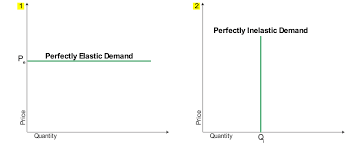
\includegraphics[width=8cm]{perfect elasticities.png}
    \end{tabular}
    \caption*{To remember which is which, just note that perfectly \underline{i}nelastic demand looks like an ``I", while perfectly \underline{e}lastic demand looks (kind of) like an ``E"}
\end{table}
\end{frame}

\begin{frame}{Graphical Understanding}
    \begin{table}[]
        \centering
        \begin{tabular}{c}
            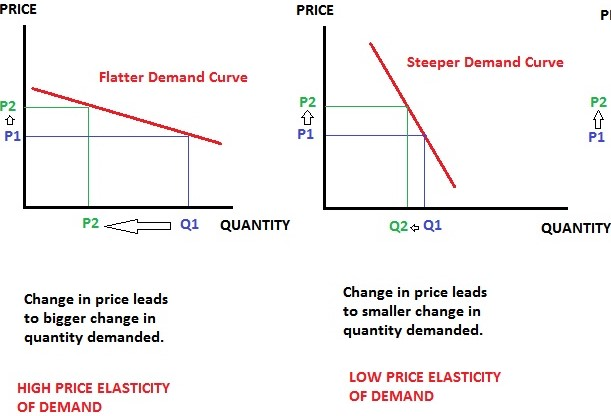
\includegraphics[width=8cm]{elastic v inelastic.jpg}
        \end{tabular}
        \caption*{Note that the same(ish) level of price change leads to larger responses in flat curves than in steep curves}
    \end{table}
\end{frame}

\end{document}